\documentclass[twocolumn,10pt]{article}
\usepackage[utf8]{inputenc}
\usepackage{graphicx}
\usepackage{amsmath}
\usepackage{amssymb}
\usepackage{geometry}
\usepackage{setspace}
\usepackage{abstract}
\usepackage{titlesec}
\usepackage[backend=biber,style=apa]{biblatex}% Changed style to apa
\usepackage[hidelinks]{hyperref}
\PassOptionsToPackage{hyphens}{url} % Pass hyphens option to url package via hyperref
\usepackage{fancyhdr} % For custom headers and footers
\usepackage{lastpage} % For page numbering in the footer
\usepackage{xcolor} % For text color
\usepackage{tabularx} % Tabularx package for better table formatting

% Set marginparwidth for todonotes
\setlength{\marginparwidth}{2cm} % Adjust the marginparwidth
\usepackage{todonotes} % TODOs
\usepackage{tcolorbox} % For colored boxes
\usepackage{caption} % For custom captions

% Fonts and typography
\usepackage{helvet} % Load the Helvetica font package
\renewcommand{\familydefault}{\sfdefault} % Set sans-serif as the default font family

% Page setup
\geometry{margin=1in}
\setstretch{1.2}
\titleformat{\section}{\bfseries\Large}{\thesection}{1em}{}
\titleformat{\subsection}{\bfseries\large}{\thesubsection}{1em}{}
\titleformat{\subsubsection}{\bfseries\normalsize}{\thesubsubsection}{1em}{}

% Add bibliography file
\addbibresource{references.bib}

% Customization to remove url date and format URLs and DOIs
\AtEveryBibitem{%
  \ifentrytype{online}{%
    \clearfield{urldate}%
    \clearfield{note}%
  }{}%
  \ifentrytype{article}{%
    \clearfield{urldate}%
  }{}%
}

\renewbibmacro*{doi+eprint+url}{%
  \printfield{doi}%
  \newunit\newblock%
  \iffieldundef{doi}{%
    \usebibmacro{eprint}%
    \newunit\newblock%
    \usebibmacro{url+urldate}}%
    {}%
}

% Customize the caption format
\captionsetup[figure]{
    labelfont=bf,           % Bold font for the label
    labelsep=space           % Use a space as the separator
}
\captionsetup[table]{
    labelfont=bf,           % Bold font for the label
    labelsep=space           % Use a space as the separator
}

% Change font size of bibliography entries
\renewcommand{\bibfont}{\fontsize{7pt}{9pt}\selectfont}% Set font size to 7pt, maybe too small. Change to 8pt if needed. Also adjust actual text size?

% Title
\title{State-of-the-Art in Visual Cortical Prostheses: Technological Advances and Future Directions}
\author{
  Marc J. Posthuma\\
  Student Number: 4413105\\
  \texttt{marc.posthuma@ru.nl}\\
  \\
  Radboud University\\
  Supervisor: Prof.\ dr.\ R.J.A.\ van\ Wezel\\
  Department of Neurobiology, Donders Centre for Neuroscience
}
\date{\today}

% Adjust page geometry to balance header and footer
\geometry{
  a4paper,
  left=20mm,
  right=20mm,
  top=30mm,
  bottom=30mm,
  headheight=60.50554pt, % Set the head height
  headsep=10pt, % Space between header and text
  footskip=30pt % Space between text and footer
}

% Custom footrule commands
\newcommand{\blackfootrule}{%
  \color{black}\makebox[\headwidth]{\rule[0.5ex]{\headwidth}{0.3pt}}%
}

\newcommand{\grayfootrule}{%
  \color{gray}\makebox[\headwidth]{\rule[0.5ex]{\headwidth}{0.3pt}}%
}

% Define fancyhdr styles
\fancypagestyle{firstpage}{
  \fancyhf{}
  \fancyhead[L]{
\includegraphics[width=5cm, keepaspectratio]{imgs/RU_logo_NL_cropped.png}}
  \fancyhead[R]{\fontsize{10}{12}\selectfont \textbf{Systematic Review in Neuroscience} \\ NWI-BM059}
  \fancyfoot[L]{\fontsize{8}{10}\selectfont \textcolor{gray}{Radboud University}}
  \fancyfoot[C]{\fontsize{8}{10}\selectfont \textcolor{gray}{\thepage\ of~\pageref{LastPage}}}
  \fancyfoot[R]{\fontsize{8}{10}\selectfont \textcolor{gray}{June 2024}}
  \renewcommand{\footrulewidth}{0.3pt}
  \renewcommand{\footrule}{\blackfootrule}
}

\fancypagestyle{rest}{
  \fancyhf{}
  \fancyhead[L]{\fontsize{8}{10}\selectfont \textcolor{gray}{Systematic Review}}
  \fancyhead[R]{\fontsize{8}{10}\selectfont \textcolor{gray}{State-of-the-Art in Visual Cortical Prostheses}}
  \fancyfoot[L]{\fontsize{8}{10}\selectfont \textcolor{gray}{Radboud University}}
  \fancyfoot[C]{\fontsize{8}{10}\selectfont \textcolor{gray}{\thepage\ of~\pageref{LastPage}}}
  \fancyfoot[R]{\fontsize{8}{10}\selectfont \textcolor{gray}{June 2024}}
  \renewcommand{\footrulewidth}{0.3pt}
  \renewcommand{\footrule}{\grayfootrule}
}

% Document
\begin{document}

\pagestyle{plain}% Default plain page style for the list of TODOs
\listoftodos% Remove this line before submission
\clearpage%To make sure the todo list is on a separate page without fancyhdr

\newpage% To make sure the todo list is on a separate page without fancyhdr

% Title and abstract
\twocolumn[
      \maketitle
      \thispagestyle{firstpage} % Apply first page style after title
      \begin{onecolabstract}
            \noindent Visual cortical prostheses represent a revolutionary technology within the field of neuro\-prosthetics, aimed at restoring vision for individuals with visual impairments through direct neural interfaces. This review systematically explores the current capabilities, limitations, and future prospects of visual cortical prostheses, with a focus on the integration of artificial intelligence (AI) to enhance functionality and effectiveness. Key topics include the optimization of phosphene patterns, real-time image processing, and comparisons with other types of prosthetic devices. The goal is to provide a comprehensive overview of the state-of-the-art in visual cortical prostheses and propose future research directions.
      \end{onecolabstract}
      \textbf{Keywords:} Visual cortical prostheses, neuroprosthetics, artificial intelligence, phosphene patterns, real-time image processing
      \vspace{1cm}
]

% Ensure first page style is applied until the first page is full
\thispagestyle{firstpage}
\section*{Introduction}\label{sec:intro}
\subsection*{Background}
Globally, blindness affects millions of people, with estimates rising from over
30 million in 2013 to 43.3 million in
2020~\parencite{stevensGlobalPrevalenceVision2013,
      bourneTrendsPrevalenceBlindness2021}. For certain types of blindness, visual
prosthetics present a promising avenue for restoring rudimentary vision through
electrical stimulation of the visual system. The concept of using bioelectrical
interfaces dates back to the 18th century, with pioneering experiments by LeRoy
in 1755 and Volta in 1800 demonstrating that electrical stimulation of the eye
can induce visual sensations.

The field of neuroprosthetics has witnessed remarkable progress, particularly
with the advent of visual cortical prostheses. These advanced devices offer hope
for restoring vision in individuals with severe visual impairments by
interfacing directly with the brain's visual cortex
(Figure~\ref{fig:schematic}). Visual cortical prostheses work by converting
visual information from the external environment into neural signals that the
brain can process, effectively bypassing damaged visual pathways. The core
technology involves the generation of phosphenes---perceived spots of light
resulting from electrical stimulation of the visual
cortex~\parencite{vandergrintenBiologicallyPlausiblePhosphene2024a}. However,
organizing these phosphenes into coherent and interpretable visual patterns
remains a significant challenge~\parencite{merabetWhatBlindnessCan2005}.

\pagestyle{rest} % Apply rest page style from here

% Schematic figure (Bio-render)
\begin{figure*}[ht!]
      \centering
      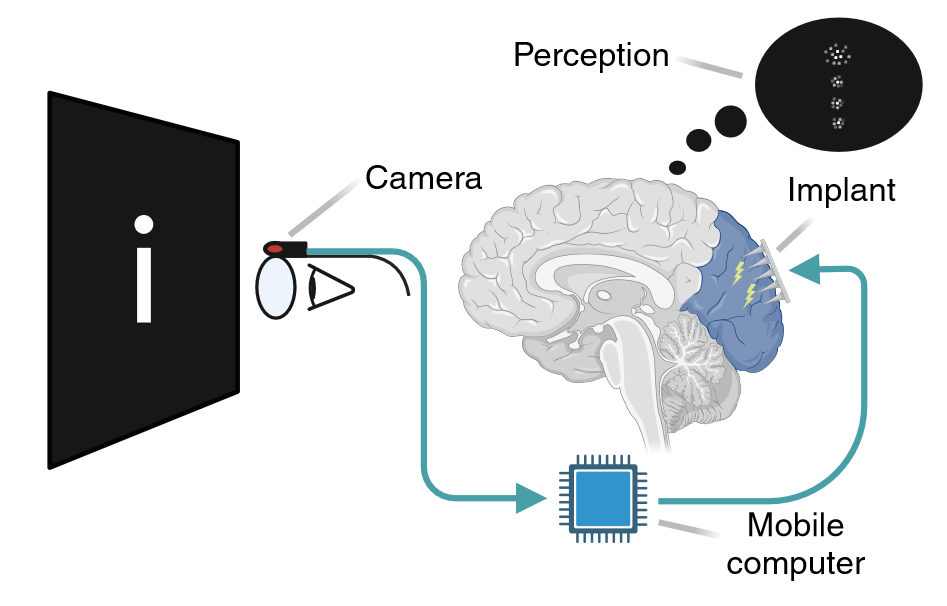
\includegraphics[width=0.7\textwidth]{imgs/visual_cortical_prothesis.png}
      \caption{| Functional schematic representation of a visual cortical
            prosthesis. The visual environment is recorded by a wearable camera
            and sent to a (wireless) mobile computer. Electrodes within a brain
            implant are then selectively activated to stimulate neurons in the
            primary visual cortex (V1). By leveraging the retinotopic
            organization of V1, a precise pattern of phosphenes is created,
            forming a coherent representation of the visual
            scene~\parencite{chenShapePerceptionHighchannelcount2020}. (Image:
            BioRender,
            \href{https://app.biorender.com/}{https://app.biorender.com/},
            accessed on 27 May 2024).}\label{fig:schematic}
\end{figure*}

AI has emerged as a pivotal element in enhancing these prosthetic systems. By
leveraging sophisticated algorithms, AI can optimize stimulation patterns to
create more naturalistic visual experiences for
users~\parencite{kriegeskorteDeepNeuralNetworks2015}. AI's role extends to real-time
image processing, allowing the prosthesis to adapt to varying visual
environments and tasks~\parencite{marblestoneIntegrationDeepLearning2016}. This
capability is crucial for developing prosthetic systems that closely mimic
natural vision, providing users with more effective and adaptable solutions. The
integration of AI not only improves the functionality of these devices but also
opens new avenues for innovation in how visual information is processed and
perceived~\parencite{gallettiCorticalConnectionsArea2001}.

This review aims to provide a comprehensive analysis of visual cortical
prostheses, focusing on the role of AI in advancing these prosthetics. By
examining current capabilities, identifying limitations, and proposing future
research directions, this work seeks to contribute to the ongoing development of
more effective and user-friendly visual prosthetic systems. Combining
technological innovation with neuroscientific insights has the profound
potential to enhance the quality of life for individuals with visual
impairments.

\subsection*{Research Question}
This review addresses the following questions:
\begin{itemize}
      \item What are the current technological advancements in visual cortical
            prostheses, particularly in electrode design, signal processing, and
            integration?
      \item How is AI leveraged to enhance visual prostheses, particularly in
            optimizing phosphene patterns and real-time image
            processing?
      \item How do visual cortical prostheses compare with other types of
            prosthetic devices?
      \item What are the functional differences between AI-enhanced prosthetic
            vision and natural visual processing within the human brain?
\end{itemize}

\subsection*{Key Articles}\label{sec:key_articles}
To ground this review, several key articles have been selected that highlight
the current state and advancements in visual cortical prostheses:
\begin{itemize}
      \item Van der Grinten et al. (2024) discuss the simulation of phosphene
            patterns for optimizing visual
            experiences~\parencite{vandergrintenBiologicallyPlausiblePhosphene2024a}.
      \item Farnum \& Pelled (2020) review the advancements in microelectronic
            devices and the integration of AI for enhanced visual
            prostheses~\parencite{farnumNewVisionVisual2020}.
      \item Grani et al. (2022) explore closed-loop stimulation strategies for
            real-time adjustments in visual
            prostheses~\parencite{graniPersonalizedClosedloopStimulation2022}.
\end{itemize}

\subsection*{Objectives}\label{sec:objectives}
The primary objectives of this review are:
\begin{itemize}
      \item To synthesize recent technological advancements in visual cortical
            prostheses.
      \item To evaluate the integration and impact of AI in enhancing these
            prosthetic systems.
      \item To compare visual cortical prostheses with other prosthetic devices
            and natural vision.
      \item To identify current limitations and propose future research
            directions.
\end{itemize}

\section*{Technological Advances}\label{sec:tech_advances}
Recent years have seen significant progress in the development of visual
cortical prostheses, driven by advancements in both hardware and software
systems. These innovations are pivotal in enhancing the functionality,
efficiency, and user experience of these devices.

\subsection*{Advancements in Biomaterials and Electrode Design}
One major area of advancement is in electrode design and fabrication.
Traditional electrodes have been limited by issues such as biocompatibility,
stability, and the ability to generate precise neural stimulation. Recent
studies have introduced novel materials and fabrication techniques that
significantly improve these aspects.

\subsubsection*{Conductive Polymers}
The development of flexible and biocompatible electrodes allows for better
integration with neural tissue, reducing the risk of damage and increasing the
longevity of the implants~\parencite{xiangFlexibleThreedimensionalElectrode2016}.
Conductive polymers have been instrumental in advancing the design and
functionality of these electrodes.

One notable conductive polymer is PEDOT:PSS (poly (3,4-ethylenedioxythiophene)
polystyrene sulfonate), which has been widely used due to its excellent
electrical conductivity, flexibility, and biocompatibility. PEDOT:PSS coatings
on electrodes improve signal transduction and reduce impedance, which enhances
the quality of neural recordings and
stimulation~\parencite{rivnayHighperformanceTransistorsBioelectronics2015}.

Another significant advancement is the use of polyaniline (PANI), a conductive
polymer known for its tunable conductivity and biocompatibility. PANI can be
chemically modified to optimize its electrical properties, making it suitable
for long-term neural interfacing applications. Its use in electrode design has
shown promising results in maintaining stable performance over extended
periods~\parencite{almuflehHighlyFlexiblePolyanilineBased2021}.

Polypyrrole (PPy) is another conductive polymer that has been extensively
studied for neural applications. PPy-based electrodes offer a unique combination
of electrical conductivity and mechanical properties that facilitate close
contact with neural tissue. Additionally, PPy can be doped with various
bioactive molecules to promote tissue integration and reduce inflammatory
responses~\parencite{zareElectroconductiveMultifunctionalPolypyrrole2021a}.

These advancements in conductive polymers are crucial for the development of
next-generation neural prostheses, offering improved performance,
biocompatibility, and longevity.

\subsubsection*{Nanotechnology}
Advances in microfabrication have enabled the creation of high-density electrode
arrays that can stimulate the visual cortex with greater precision, offering the
potential for more detailed and coherent visual
experiences~\parencite{ryuSpatiallyConfinedResponses2020}.

Nanotechnology has introduced several innovative approaches to enhance the
performance and integration of electrodes in visual cortical prostheses. One
such approach is the use of carbon nanotubes (CNTs), which possess exceptional
electrical conductivity and mechanical strength. CNTs can be incorporated into
electrode designs to improve signal transmission and reduce impedance, thereby
enhancing the quality of neural
stimulation~\parencite{alegretThreeDimensionalConductiveScaffolds2018}.

Another promising implementation is the use of graphene, a two-dimensional
material known for its outstanding electrical and thermal properties.
Graphene-based electrodes have shown excellent biocompatibility and flexibility,
which are crucial for long-term implantation and stable neural interfaces. The
incorporation of graphene into electrode arrays allows for better integration
with neural tissue and more precise stimulation of the visual
cortex~\parencite{luGraphenebasedNeurotechnologiesAdvanced2018}.

Additionally, gold nanostructures have been utilized to enhance electrode
performance. Gold nanoparticles and nanowires can be used to modify the surface
of electrodes, increasing their surface area and improving their electrical
properties. This modification can lead to more efficient charge transfer and
lower stimulation thresholds, resulting in more effective and reliable neural
stimulation~\parencite{zareGoldNanostructuresSynthesis2022}.

These nanotechnology-based advancements are paving the way for the development
of more sophisticated and effective visual cortical prostheses, providing users
with improved visual experiences and greater functionality.

\subsubsection*{3D Printing}
Recent advancements in 3D printing has significantly impacted the field of
visual cortical prostheses, particularly in the fabrication of electrodes. 3D
printing offers unparalleled precision and customization capabilities, allowing
for the creation of complex and highly detailed electrode arrays that can be
tailored to the unique anatomical features of individual
patients~\parencite{guoImplantableLiquidMetalbased2017}.

This technology enables the production of electrodes that conform to the
specific geometry of the cortical surface, improving contact and integration
with neural tissue, thereby enhancing the accuracy of neural stimulation and
minimizing potential damage to surrounding
tissues~\parencite{liuSoftElasticHydrogelbased2019}. Advances in 3D printing
materials, including biocompatible and conductive inks, have improved the
performance and longevity of printed electrodes, providing the necessary
electrical properties while maintaining compatibility with neural tissue.

Additionally, the ability to rapidly prototype and produce electrodes using 3D
printing reduces manufacturing time and cost, facilitating quicker iterations
and refinements in electrode design, which accelerates the development
process~\parencite{zhangClimbinginspiredTwiningElectrodes2019}. Recent studies
have demonstrated the potential in creating flexible and biocompatible
electrodes, advancing the state-of-the-art in visual cortical prostheses.

\subsection*{Improved Signal Processing and Integration}
Advances in signal processing and integration have been crucial in enhancing the
performance and functionality of visual cortical prostheses. High-resolution
imaging techniques and sophisticated signal processing algorithms have
significantly improved the precision and reliability of these devices.

\subsubsection*{High-Resolution Imaging}
High-resolution imaging techniques have played a pivotal role in the advancement
of visual cortical prostheses by providing detailed maps of the brain's cortical
structures. These techniques allow for more precise placement and targeting of
electrodes, which is essential for effective neural stimulation.

Optical Coherence Tomography (OCT) is one such high-resolution imaging technique
that has been extensively used in neural prosthetics. OCT provides
cross-sectional images of the brain's surface, enabling detailed visualization
of cortical layers and structures. This level of detail allows for the precise
placement of electrodes, improving the effectiveness and safety of neural
stimulation~\parencite{xieUseOpticalCoherence2022}.

Functional Magnetic Resonance Imaging (fMRI) provides high-resolution images of
brain activity by detecting changes associated with blood flow. This imaging
technique is valuable for mapping functional areas of the brain, ensuring that
electrodes are placed in regions that will yield the most beneficial outcomes
for the user~\parencite{landelleInvestigatingHumanSpinal2021}.

Two-photon microscopy allows for deep imaging of living brain tissue with high
spatial resolution. This technique is particularly useful for observing the
interactions between electrodes and neural tissue over time, providing insights
that can guide the design and optimization of electrode
arrays~\parencite{yangIntegratedMicroprismMicroelectrode2024}.

Furthermore, the development of NIR-II semiconducting polymers has enhanced in
vivo high-resolution imaging capabilities. These polymers offer excellent
penetration depth and spatial resolution, which are critical for accurate
diagnostics and therapeutic applications in neural prosthetics~\parencite{wangRecentProgressSecond2023,kangNIRIISemiconductingPolymers2023}.

Deep learning techniques have also been employed to enhance the resolution of
confocal fluorescence microscopy. By using generative models, these techniques
improve the learning ability of imaging systems in the frequency domain,
resulting in significantly higher resolution images that are essential for
detailed neural mapping~\parencite{huangEnhancingImageResolution2023}.

These high-resolution imaging techniques are integral to the development of more
precise and effective visual cortical prostheses, facilitating better
integration and performance of these devices.

\subsubsection*{Wireless Communication}
Additionally, innovations in wireless technology have enabled the development of
untethered visual cortical prostheses. Wireless systems eliminate the need for
external wires, which not only improves the comfort and aesthetics of the
prostheses but also reduces the risk of infections and mechanical failures.
Advancements in wireless power transfer and data communication have made it
possible to deliver sufficient power and high-fidelity signals to the implants,
ensuring reliable and efficient
operation~\parencite{rosenfeldTissueResponseChronically2020}.

Recent advancements include the development of biphasic quasistatic brain
communication (BP-QBC), a technique that significantly reduces power consumption
while maintaining high data transfer rates. This method leverages
electro-quasistatic signaling to create a low-power, broadband communication
channel between wireless neural implants and external devices, offering a
promising solution for energy-efficient and high-speed data transmission in
neural prosthetics~\parencite{chatterjeeBiphasicQuasistaticBrain2023}.

Another innovative approach is the use of feed-forward neural networks to
improve the control of brain-machine interfaces. This simpler neural network
architecture enhances the speed and accuracy of prosthetic control by more
closely mimicking the natural communication pathways between the brain and the
body. Such advancements not only improve the functionality of prosthetic devices
but also enhance their usability for individuals with paralysis or limb
loss~\parencite{willseyRealtimeBrainmachineInterface2022}.

Moreover, multidimensional graph neural networks (GNNs) have been employed to
optimize wireless communication policies in neural prosthetics. These networks
use graph-based representations to manage complex data transmission scenarios,
improving the efficiency and reliability of wireless communication between
implants and external devices~\parencite{liuMultidimensionalGraphNeural2024}.

These advancements in wireless communication technology are crucial for the
development of next-generation visual cortical prostheses, providing users with
more seamless and reliable neural interfaces.

\subsection*{Software and Algorithmic Enhancements}
On the software side, the integration of artificial intelligence (AI) has
revolutionized the way visual information is processed and interpreted by
prosthetic systems. AI algorithms, particularly those based on deep learning,
have been employed to optimize stimulation patterns and enhance image processing
capabilities. These algorithms can learn from vast amounts of data to improve
the accuracy and efficiency of visual signal conversion, making the visual
experiences more naturalistic and adaptable to different
environments~\parencite{romeniMachineLearningFramework2021}.

\subsubsection*{Real-Time Data Processing}
Real-time data processing is pivotal in the functionality of visual cortical
prostheses. It enables the seamless translation of visual information from the
external environment into neural signals that can be interpreted by the brain's
visual cortex.

A key aspect of real-time data processing involves the integration of high-speed
computing systems capable of handling large volumes of visual data with minimal
latency~\parencite{nurmikkoChallengesLargeScaleCortical2020}. The processing
pipeline typically includes capturing visual information via cameras,
preprocessing the data to reduce noise and enhance relevant features, and
converting this data into neural stimulation patterns.

Edge computing plays a crucial role in this pipeline by performing data
processing closer to the data source. This reduces latency and enhances the
responsiveness of the prosthetic system, which is particularly important for
real-time applications such as navigation in dynamic
environments~\parencite{wangDeepLearningEdge2020}. By offloading computational
tasks from centralized servers to local devices, edge computing ensures that
visual data is processed swiftly, enabling immediate feedback to the user.

Another important component is the use of adaptive algorithms that can
dynamically adjust to changes in the visual environment. These algorithms
leverage feedback from the user's interactions with the prosthetic system to
continuously improve accuracy and
effectiveness~\parencite{pio-lopezVisualCorticalProsthesis2021b}. For example,
real-time adjustments can be made to the stimulation patterns based on
environmental factors such as lighting conditions and the presence of moving
objects, ensuring that the visual output remains consistent and
coherent~\parencite{fylstraHumanprosthesisCooperationCombining2022}.

Additionally, advancements in sensor technology have significantly contributed
to real-time data processing capabilities. High-resolution cameras and depth
sensors provide detailed visual information, which is essential for generating
precise and informative neural signals. These sensors can capture a wide range
of visual cues, including color, depth, and motion, which are then processed to
create a comprehensive visual experience for the
user~\parencite{rueckauerExperiencingProstheticVision2022}.

Real-time data processing also benefits from the development of specialized
hardware accelerators, such as Graphics Processing Units (GPUs) and Field
Programmable Gate Arrays
(FPGAs)~\parencite{springerOnDeviceDeepLearning2021,fengDesignOnlineBrainComputer2020}
These devices are optimized for parallel processing tasks and can handle the
intensive computational demands of real-time visual data processing. By
utilizing these hardware accelerators, visual cortical prostheses can achieve
the necessary processing speeds to provide immediate and accurate visual
feedback.

In summary, real-time data processing in visual cortical prostheses involves a
combination of high-speed computing, edge computing, adaptive algorithms,
advanced sensors, and specialized hardware accelerators. These systems work
together to ensure that visual information is processed and transmitted to the
brain without noticeable delays, creating a natural and effective visual
experience for users. This seamless integration of hardware and software
components is crucial for the ongoing development and enhancement of visual
prosthetic systems.

% Add the summary box at the end of the Technological Advances section
\begin{figure*}[ht!]
      \begin{tcolorbox}[
                  title=Technological Advances in Visual Cortical Prostheses,
                  colframe=gray!30, % Border color
                  colback=gray!20, % Background color
                  coltitle=white, % Title color
                  colbacktitle=gray!50, % Title background color
                  fonttitle=\bfseries,
                  sharp corners=all,
                  width=\textwidth,
                  boxrule=1.5pt % Border width
            ]
            \fontsize{8pt}{10pt}\selectfont % Set the font size directly
            \begin{itemize}
                  \item \textbf{Advancements in Biomaterials and Electrode Design}
                        \begin{itemize}
                              \item \textbf{Conductive Polymers:} PEDOT:PSS, Polyaniline (PANI), Polypyrrole (PPy)
                              \item \textbf{Nanotechnology:} Carbon Nanotubes (CNTs), Graphene, Gold Nanostructures
                              \item \textbf{3D Printing:} Customizable and high-precision electrode arrays
                        \end{itemize}

                  \item \textbf{Improved Signal Processing and Integration}
                        \begin{itemize}
                              \item \textbf{High-Resolution Imaging:} Optical Coherence Tomography (OCT), Functional Magnetic Resonance Imaging (fMRI), Two-photon microscopy, NIR-II semiconducting polymers
                              \item \textbf{Wireless Communication:} Biphasic Quasistatic Brain Communication (BP-QBC), Feed-forward Neural Networks, Graph Neural Networks (GNNs)
                        \end{itemize}

                  \item \textbf{Software and Algorithmic Enhancements}
                        \begin{itemize}
                              \item \textbf{Real-Time Data Processing:} Edge computing, adaptive algorithms, advanced sensors, hardware accelerators (GPUs and FPGAs)
                        \end{itemize}

                  \item \textbf{Other Functional Improvements}
                        \begin{itemize}
                              \item \textbf{Closed-Loop Feedback Systems:} Dynamic adjustment of stimulation parameters
                              \item \textbf{Multi-Modal Sensory Integration:} Incorporation of auditory and tactile feedback
                              \item \textbf{Neuroplasticity and Rehabilitation:} Training protocols to enhance neural integration
                        \end{itemize}
            \end{itemize}
      \end{tcolorbox}
      % \caption{Summary of key technological advancements in the development of
      %       visual cortical prostheses, highlighting improvements in biomaterials,
      %       signal processing, software, and functional
      %       integration.}\label{fig:advances_vcp}
\end{figure*}

\subsection*{Other Functional Improvements}
In recent years, there have been several significant functional improvements in
visual cortical prostheses. These advancements include the development of
closed-loop feedback systems, the integration of multi-modal sensory input, and
the application of neuroplasticity principles in rehabilitation programs.

\subsubsection*{Closed-Loop Feedback Systems}
Another significant advancement is the implementation of closed-loop systems in
visual cortical prostheses. These systems continuously monitor neural feedback
to adjust stimulation parameters in real-time, thereby enhancing the precision
and effectiveness of visual restoration. Closed-loop systems mimic the natural
feedback mechanisms of the human visual system, providing a more responsive and
user-friendly experience. Recent research has demonstrated the efficacy of these
systems in improving the visual outcomes for users, as they can dynamically
adapt to changes in the environment and the user's neural
responses~\parencite{leviEditorialClosedLoopSystems2018}.

\subsubsection*{Multi-Modal Sensory Integration}
The integration of multi-modal sensory input is another promising development in
this field. By incorporating inputs from other senses, such as auditory or
tactile feedback, visual cortical prostheses can provide a more holistic sensory
experience. This multi-modal approach leverages the brain's ability to integrate
information from different sensory modalities, potentially enhancing the overall
perceptual experience and aiding in the interpretation of visual
scenes~\parencite{wanArtificialSensoryNeuron2020}.

\subsubsection*{Neuroplasticity and Rehabilitation}
Advancements in understanding neuroplasticity have led to improved
rehabilitation strategies for users of visual cortical prostheses.
Neuroplasticity refers to the brain's ability to reorganize itself by forming
new neural connections. Rehabilitation programs that stimulate neural
reorganization can enhance the integration and functionality of prosthetic
devices. These programs often involve specific training protocols designed to
help users better interpret and respond to visual stimuli, ultimately improving
their overall visual experience.

\section*{AI Integration}\label{sec:ai_integration}
The integration of AI in visual prosthesis systems is focused on how deep
learning algorithms enhance visual data processing, optimize phosphene patterns,
and emulate normal brain processing. Figure~\ref{fig:simulator_framework}
provides an overview of a Visual Prosthesis Simulation Framework based
on~\parencite{deruytervansteveninckEndtoendOptimizationProsthetic2022}. This
framework employs AI to simulate and predict how users perceive visual
information through a prosthetic device. By integrating deep learning
algorithms, the system can accurately replicate and enhance visual experiences.

The functional process of a visual cortical prosthesis in this framework is an
end-to-end process that includes three main components: an encoder, a phosphene
simulator, and a decoder. The encoder processes the input image to generate a
stimulation protocol, which determines the intensity of stimulation for each
electrode. The phosphene simulator translates this protocol into a simulated
phosphene vision (SPV) representation, incorporating factors like distortions in
phosphene positions and brightness variations. Finally, the decoder reconstructs
the input image from the SPV representation, ensuring accurate interpretation of
the encoded information.

Optimization is a critical aspect, involving automated and tailored adjustments
to achieve the best visual reconstruction. Task-specific optimization is
implemented by using different loss functions, guiding the network to preserve
relevant information. Constraints such as sparsity can be incorporated to
minimize adverse effects of electrical stimulation. The modular design allows
the system to adapt to practical, medical, or biophysical limitations.

These different types of neural networks include: CNNs for image recognition,
RNNs for temporal data processing, GANs for generating realistic visual
patterns, and GNNs for understanding complex spatial relationships. These
algorithms collectively improve the capability for image translation, object
recognition, and scene interpretation.

% Diagram figure (inkscape)
\begin{figure*}[ht!]
      \centering
      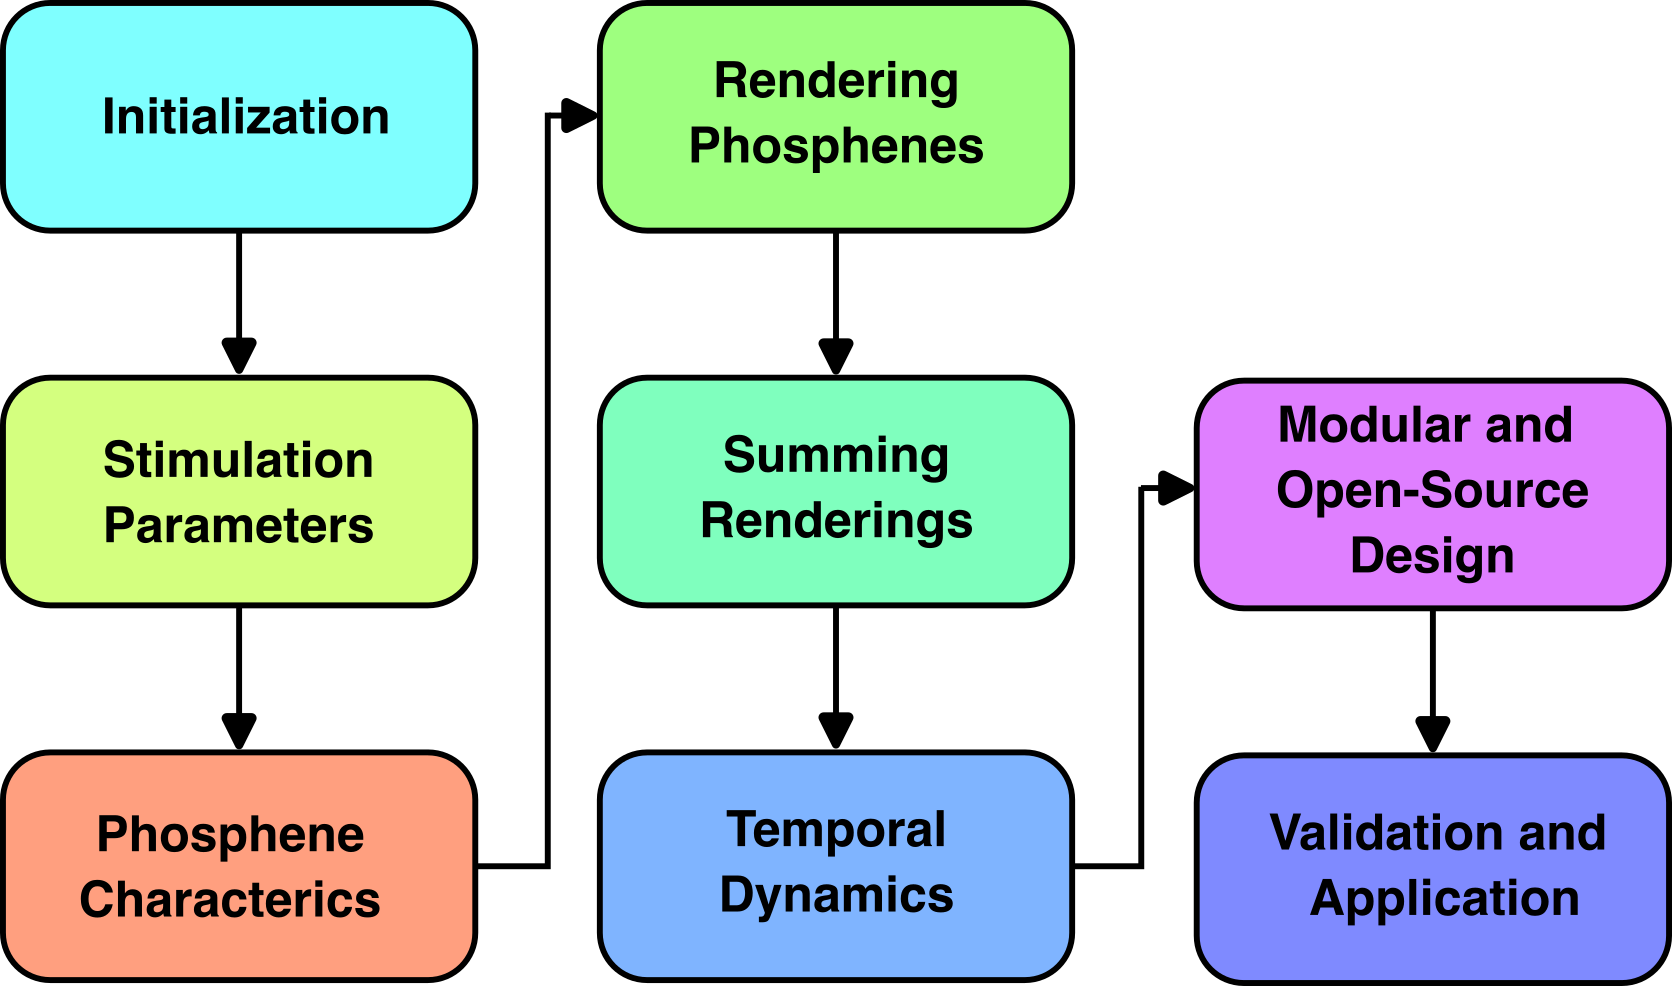
\includegraphics[width=0.6\textwidth]{imgs/block_diagram_vis_prost.png}
      \caption{| Overview of a Visual Prosthesis Simulation Framework. The
            simulator is initialized with electrode locations on a visuotopic
            map of the visual cortex (V1), representing the spatial organization
            of the visual field. For each frame, it processes stimulation
            parameters such as amplitude, pulse width, and frequency for each
            electrode. Using these parameters and electrode locations, it
            estimates phosphene characteristics, which are rendered on a visual
            field map considering cortical magnification and activation
            thresholds. Individual phosphene renderings are summed to produce
            the simulated prosthetic percept. Temporal dynamics, including
            delayed onset and offset of perception, are modeled using a leaky
            integrator. The simulator's modular and open-source design,
            implemented in Python with PyTorch for example, allows for fast GPU
            computations and easy integration with external
            software~\parencite{deruytervansteveninckEndtoendOptimizationProsthetic2022}.
            It is validated through computational and behavioral experiments,
            incorporating neurophysiological and clinical findings to ensure
            biological plausibility.}\label{fig:simulator_framework}
\end{figure*}

\subsection*{Deep Learning Algorithms in Prosthetic Vision}
So why are deep learning algorithms essential for prosthetic vision?

\todo[inline]{Check if the citations are in the right spots.}

\subsubsection*{Predictive Modeling}
Predictive modeling plays a crucial role in prosthetic vision by leveraging
various deep learning algorithms to enhance visual perception for users. These
models are designed to predict and interpret visual inputs, creating a seamless
and coherent visual experience. By utilizing large datasets and advanced neural
network architectures, predictive modeling enables the prosthetic system to
anticipate and adapt to dynamic visual environments. Key deep learning
algorithms are employed in predictive modeling, including
Convolutional Neural Networks (CNNs), Recurrent Neural Networks (RNNs),
Generative Adversarial Networks (GANs), and Multidimensional Graph Neural
Networks (GNNs), each contributing uniquely to improving the functionality and
performance of visual cortical prostheses.

\subsubsection*{Convolutional Neural Networks (CNNs)}
CNNs are employed to process and classify visual inputs, enhancing the ability
of the prosthetic system to interpret complex visual scenes and improve object
recognition capabilities. CNNs are particularly effective at identifying spatial
hierarchies in images through layers of convolutions that capture features like
edges, textures, and shapes. By training on large datasets, CNNs learn to
recognize a wide range of objects and scenes, enabling the prosthetic system to
provide users with detailed and accurate visual
information~\parencite{petrosyanDecodingInterpretingCortical2021a}. This improves the
user's ability to navigate and interact with their environment by providing
clearer and more recognizable visual
cues~\parencite{maheswaranathanInterpretingRetinalNeural2023}.

\subsubsection*{Recurrent Neural Networks (RNNs)}
RNNs, including LSTM (Long Short-Term Memory) networks, are used to handle
sequential data, making it possible to maintain temporal continuity in visual
perception and improve the user's ability to track moving objects. Unlike CNNs,
which focus on spatial relationships, RNNs excel at processing temporal
sequences. They retain information over time, allowing them to predict future
frames based on past visual data. This capability is essential for maintaining a
continuous and stable visual experience, especially when tracking dynamic scenes
or moving objects, thereby enhancing the user's perception of motion and
improving their ability to react to changes in their
environment~\parencite{nayebiRecurrentConnectionsPrimate2022, liaoBridgingGapsResidual2016}.

\subsubsection*{Generative Adversarial Networks (GANs)}
GANs are utilized to generate realistic phosphene patterns by training on large
datasets of visual scenes, improving the fidelity and natural appearance of the
visual output. A GAN consists of two neural networks, a generator and a
discriminator, which are trained together in a competitive process. The
generator creates synthetic images that the discriminator attempts to
distinguish from real images. Through this adversarial training, GANs learn to
produce high-quality, realistic images that can be used to simulate
phosphenes—patterns of light perceived by the visual
cortex~\parencite{goodfellowGenerativeAdversarialNetworks2020,elnabawyPVGANGenerativeAdversarial2022}.
This enhances the naturalness and coherence of the visual scenes presented to
the user, making the prosthetic vision more similar to natural sight.

\subsubsection*{Multidimensional Graph Neural Networks (GNNs)}
GNNs are leveraged to model and interpret complex relationships within
multidimensional data, enhancing the system's ability to understand and process
spatial and relational information. GNNs extend traditional neural networks by
operating on graph-structured data, which can represent the spatial
relationships between objects in a scene. This allows the prosthetic system to
better understand the context and interactions within the visual input. By
capturing these intricate relationships, GNNs improve the prosthetic's ability
to recognize patterns, structures, and spatial hierarchies, leading to more
accurate and context-aware visual perception. This is particularly useful in
complex environments where understanding the spatial arrangement of objects is
crucial for navigation and
interaction~\parencite{subramanianGraphConvolutionalNetworks2020,wuComprehensiveSurveyGraph2021}.

\section*{Comparison with Other Visual Systems}\label{sec:comparison}
Cortical prosthetics offer a unique approach to restoring vision compared to
earlier retinal and optic nerve implants. Devices by companies like the
\textit{PRIMA system} and \textit{IRIS} systems by Pixium-Vision or the
\textit{Orion} and \textit{ARGUSII} (FDA-approved) by Second Sight Medical
Products Inc have already proven their merit. However, cortical prostheses are
distinguished by their downstream positioning, which provides substantial
rehabilitative potential for individuals who are blind or visually impaired,
especially when retinal or optic nerve prostheses are
ineffective~\parencite{tzekovGabelEdArtificial2020}. These implants also allow
for the longest therapeutic intervention window. Instead of complete neural
degeneration, post-injury compensatory plasticity mechanisms recruit neurons
from other cortical regions, enabling effective stimulation well beyond the
onset of injury or disease~\parencite{beyelerLearningSeeAgain2017}.

\begin{table*}[ht!]
      \centering
      \caption{| Comparison of Cortical, Retinal, and Optic Nerve Prostheses}\label{tab:prostheses_comparison}
      \begin{tabularx}{\textwidth}{|X|X|X|X|}
            \hline
            \textbf{Feature}                  & \textbf{Cortical Prostheses}                                                       & \textbf{Retinal Prostheses}                                                    & \textbf{Optic Nerve Prostheses}                                 \\ \hline
            \textbf{Target Area}              & Visual cortex                                                                      & Retina                                                                         & Optic nerve                                                     \\ \hline
            \textbf{Surgical Invasiveness}    & Highly invasive (brain surgery)                                                    & Moderately invasive (eye surgery)                                              & Moderately invasive (requires access to the optic nerve)        \\ \hline
            \textbf{Applicability}            & Suitable for severe visual impairment with retinal or optic nerve damage           & Best for retinal degenerative diseases with some functional retinal cells      & Suitable for optic nerve damage with functional retinal cells   \\ \hline
            \textbf{Mechanism}                & Direct stimulation of the visual cortex                                            & Stimulation of remaining functional retinal cells                              & Stimulation of the optic nerve fibers                           \\ \hline
            \textbf{Therapeutic Window}       & Longest, can be effective long after onset of blindness                            & Requires some residual retinal function                                        & Depends on the extent of optic nerve damage                     \\ \hline
            \textbf{Technological Complexity} & High (phosphene organization and neural plasticity)                                & Moderate (retinal cell stimulation)                                            & High (complexity in targeting optic nerve fibers)               \\ \hline
            \textbf{Advantages}               & Broad applicability, effective for extensive damage, leverages cortical plasticity & Less invasive, established success in specific diseases, direct visual pathway & Can target optic nerve damage directly, bypasses retinal issues \\ \hline
            \textbf{Disadvantages}            & Highly invasive surgery, complex visual pattern organization                       & Limited to retinal functionality, less effective with severe damage            & Invasive, technical challenges in precise nerve stimulation     \\ \hline
      \end{tabularx}
\end{table*}

\subsection*{Comparison with Retinal Prostheses}
How do these new systems compare to existing visual prostheses?

\subsection*{Comparison with Optic Nerve Prostheses}

\subsection*{Comparison with Natural Vision}
Plasticity and perceptual learning, how are these phenomena involved in learning
to see again with a prosthesis?

\section*{Limitations and Challenges}\label{sec:limitations}
Details current drawbacks, biocompatibility issues, and areas requiring
improvement in visual cortical prosthesis technology. Is the vision from ARGUSII
for instance, any good? How do the number of electrodes matter in visual
resolution in the experience of the user?

\section*{Future Perspectives}\label{sec:future}
Provides a comprehensive overview of the current state and future potential of
visual cortical prostheses, highlighting technological capabilities, AI
integration, and challenges.

\subsection*{Clinical Applications}
A caveat is the invasive nature of these cortical devices, which require
surgical implantation.

\begin{itemize}
      \item Broader and more diverse clinical trials to assess long-term efficacy
            and safety.
      \item Exploration of personalized prosthetic solutions tailored to
            individual neural architectures.
\end{itemize}

\subsection*{Ethical and Societal Implications}
\begin{itemize}
      \item Considerations of the ethical implications of advanced neural
            interfacing.
      \item Societal impact and accessibility of such technology for individuals
            with visual impairments.
\end{itemize}

\section*{Conclusion}\label{sec:conclusion}
In conclusion, the technological advancements in electrode design,
microfabrication, artificial intelligence, closed-loop systems, wireless
technology, and multi-modal sensory integration are significantly advancing the
field of visual cortical prostheses. These innovations are crucial for
developing more effective, reliable, and user-friendly devices that can better
restore vision for individuals with severe visual impairments. Continued
research and development in these areas promise to further enhance the
capabilities and accessibility of visual cortical prostheses, paving the way for
their widespread clinical application.

\printbibliography%

\end{document}
